\chapter{Reißverschlussverfahren}
\section{Reißverschlussverfahren - StVO}
\begin{center}
	\textit{"' Ist auf Straßen mit mehreren Fahrstreifen für eine Richtung das durchgehende Befahren eines Fahrstreifens nicht möglich oder endet ein Fahrstreifen, ist den am Weiterfahren gehinderten Fahrzeugen der Übergang auf den benachbarten Fahrstreifen in der Weise zu ermöglichen, dass sich diese Fahrzeuge \textbf{unmittelbar vor Beginn der Verengung jeweils im Wechsel} nach einem auf dem durchgehenden Fahrstreifen fahrenden Fahrzeug einordnen können (Reißverschlussverfahren)."'} - StVO \S 7 Absatz 4
\end{center}
\textbf{Vorteile:} 
\begin{itemize}
	\item relativ einfach zu verstehendes Verfahren
\item "'faires Verfahren"': Die Spuren wechseln sich beim Durchfahren der Engstelle ab, wodurch man auf beiden Spuren ungefähr gleichschnell die Engstelle passiert.
\item Die Fahrbahn wird bis zur Engstelle optimal ausgelastet.
\item Das Verfahren hat sich in den letzen Jahren bewährt und jeder Autofahrer kennt die Theorie aus der Fahrschule.
\end{itemize}
\textbf{Nachteile:}
\begin{itemize}
	\item In der Praxis sortieren sich viele Autofahrer schon weit vor Ende des Fahrstreifens ein.
\item Bei großem Verkehrsaufkommen kann der Verkehr zum Stehen kommen.
\item Autofahrer müssen anhalten, um andere Autofahrer reinzulassen.
\end{itemize}
\newpage

\section{Reißverschlussverfahren - Alternative}
\textbf{Idee:} Je höher die Geschwindigkeit desto mehr Autos können die Engstelle innerhalb eines Zeitraums passieren. Das alternative Einfädelungverfahren (Abb. \ref{fig:alternative}) verfolgt das Ziel, dass möglichst kein Auto stehenbleiben muss, und somit kein Stau entsteht. Hierbei wird die Verengung bereits früher als normal angekündigt, damit das fahrbahnwechselnde Auto genug Zeit hat, sich eine Lücke zu suchen. Hierbei gilt die Regel, dass die erstbeste Lücke genutz wird. Hat das fahrbahnwechselnde Auto eine geeignete Lücke gefunden sortiert es sich ein, indem es halb auf die andere Spur wechselt. Dadurch wird sichergestellt, dass der Platz für das Auto freigehalten wird und gleichzeitig verhindert, dass ein von hinten kommendes Auto noch überholt. \\\\
\textbf{Vorteile:} 
\begin{itemize}
	\item Die Autos sind bereits vor der Engstelle einsortiert, wodurch kein Auto zum Stehen kommt.
\item Der Verkehrsfluss wird nicht unterbrochen.
\end{itemize}
\textbf{Nachteile:}
\begin{itemize}
	\item Es werden nicht alle Lücken optimal genutzt.
\item Bei hoher Verkehrsdichte kann es vorkommen, dass nicht genug Lücken vorhanden sind, bis die Engstelle erreicht wird.
\item Eine Änderung des Reißverschlussverfahrens würden hohe Kosten verursachen, da man die neue Regel verbreiten muss.
\item Nur bei Baustellen gut nutzbar, bei Hindernissen wie einem Unfall jedoch schwer umsetzbar, weil keine frühzeitige Ankündigung möglich ist.
\end{itemize}
\begin{figure}
	\centering
	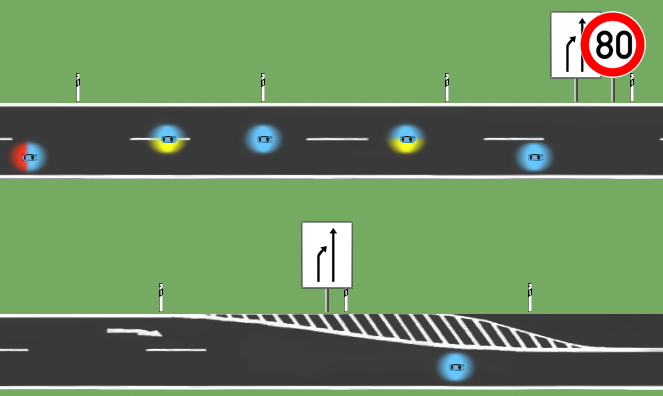
\includegraphics[width=0.7\linewidth]{images/Alternative}
	\caption{Alternatives Reißverschlussverfahren}
	\label{fig:alternative}
\end{figure}
